
\documentclass[aspectratio=169]{beamer}
\usetheme{Boadilla}

\usepackage{qrcode}

\usepackage[utf8]{inputenc}       % Codificação de entrada
\usepackage[T1]{fontenc}          % Codificação de saída
\usepackage[portuguese]{babel}   % Idioma
\usepackage{XCharter}             % Fonte principal
\AtBeginDocument{\fontsize{12}{12}\selectfont}

%\usepackage{geometry}
%\geometry{papersize={210mm,150mm}}
\usepackage{tikz}
\usepackage{pgf-pie} % necessário para gráficos de pizza

\usepackage{color}
\usepackage{graphicx}
\usepackage{amsmath, amssymb, amsfonts}
\usepackage{bm}
\usepackage{booktabs}
\usepackage{multirow}
\usepackage{caption}
\usepackage{subfigure}
\usepackage{wrapfig}
\usepackage{multicol}
\usepackage{sidecap}
\usepackage{tikz}
\usepackage{listings}
\usepackage{siunitx}
\usepackage{pdfpages}
\usepackage{float}
\usepackage{hyperref}
\usepackage{academicons}
\usepackage{setspace}

\newcommand{\eng}[1]{\textsl{#1}}
\newcommand{\cod}[1]{\texttt{#1}}

\usepackage{tikz}
\usetikzlibrary{shapes.geometric, arrows, positioning}

% Definição de estilos para o fluxograma
\tikzstyle{startstop} = [ellipse, rounded corners, minimum width=2cm, minimum height=0.8cm, text centered, draw=black, fill=gray!20]
\tikzstyle{process} = [rectangle, minimum width=3.5cm, minimum height=1cm, text width=4.5cm, text centered, draw=black, fill=white]
\tikzstyle{decision} = [diamond, aspect=2, minimum width=3cm, minimum height=1cm, text centered, draw=black, fill=white]
\tikzstyle{arrow} = [thick,->,>=stealth]

% Definição de cores profissionais
\definecolor{mipsblue}{RGB}{50, 90, 120}
\definecolor{mipsred}{RGB}{150, 30, 30}

\title[Arquitetura de Computadores]{\huge  Experimento 1} %note that the optional arg in '[]' are displayed in the left column throughout the complete presentation
% adapt accordingly
% e.g., M.Sc. Intermediate Thesis Report
% or     B.Sc. Intermediate Thesis Report


\author[Prof. Dr. Oscar Eduardo Anacona Mosquera]{Prof. Dr. Oscar Eduardo Anacona Mosquera \newline\newline 
	\scriptsize{oscar.mosquera@ufmt.br}
}%note that the optional arg in '[]' are displayed in the left column throughout the complete presentation



\AtBeginSection[]
{
	\begin{frame}{Sumário}
		\tableofcontents[currentsection]
	\end{frame}
}


\begin{document}

	\begin{frame}[plain]
		\titlepage
	\end{frame}
	
	\begin{frame}{Sumário}
		\tableofcontents
	\end{frame}
	
\begin{frame}{Objetivo do Experimento}
	\begin{itemize}
		\item Usando a placa DE0 nano.
		\item Implementar duas portas AND em paralelo.
		\item Entradas: Chaves \textbf{SW[0]} até \textbf{SW[3]}.
		\item Saídas: \textbf{LED[0]} e \textbf{LED[1]}.
		\item Fluxo: Esquemático $\rightarrow$ VHDL $\rightarrow$ Testbench $\rightarrow$ Simulação.
	\end{itemize}
	\begin{figure}
		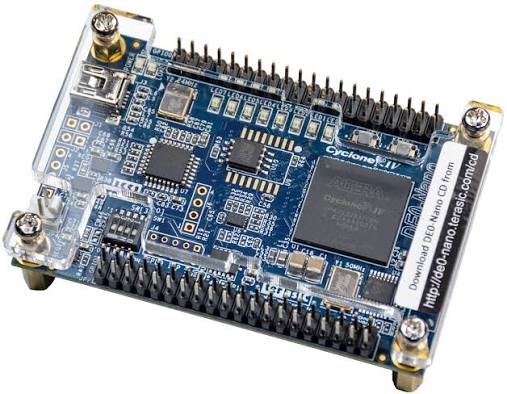
\includegraphics[width=0.4\textwidth]{Figs/placa.jpg}
	\end{figure}
\end{frame}

% --- SLIDE 2 ---
\begin{frame}{Passo 1: Hardware via Esquemático (.bdf)}
	\begin{enumerate}
		\item Abra o Quartus II 13.0.
		\item Crie um novo arquivo \textbf{Block Diagram/Schematic File}.
		\item Adicione duas portas \textit{and2}.
		\item Adicione 4 \textit{input pins} (SW[0..3]) e 2 \textit{output pins} (LED[0..1]).
		%\item Salve e defina como \textbf{Set as Top-Level Entity}.
	\end{enumerate}
	\begin{figure}
		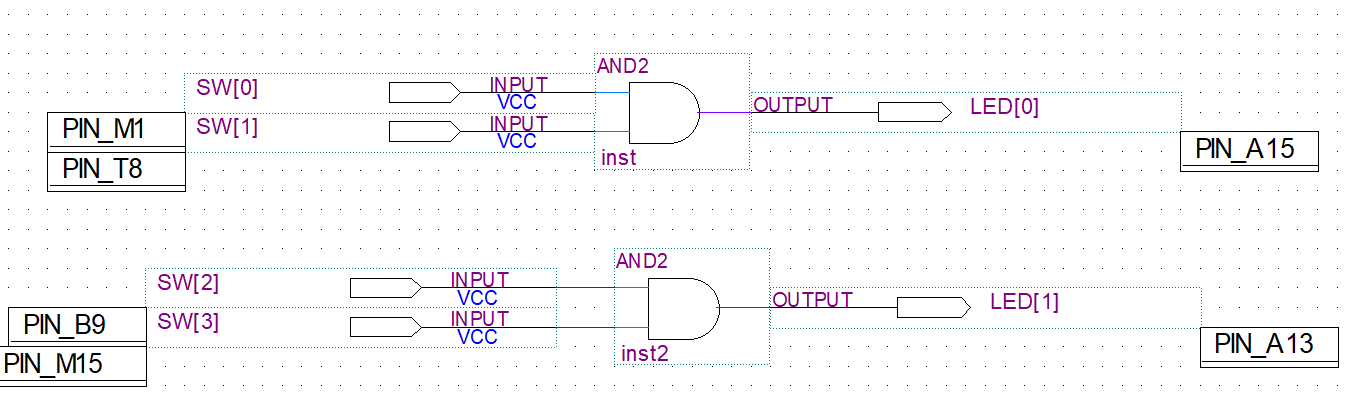
\includegraphics[width=0.6\textwidth]{Figs/tut_fig04.png}
	\end{figure}
\end{frame}



\begin{frame}{Passo 1: Hardware via Esquemático (.bdf)}
	\begin{enumerate}
		%\item Abra o Quartus II 13.0.
		%\item Crie um novo arquivo \textbf{Block Diagram/Schematic File}.
		%\item Adicione duas portas \textit{and2}.
		%\item Adicione 4 \textit{input pins} (SW[0..3]) e 2 \textit{output pins} (LED[0..1]).
		\item Salve e defina como \textbf{Set as Top-Level Entity}.
	\end{enumerate}
	\begin{figure}
		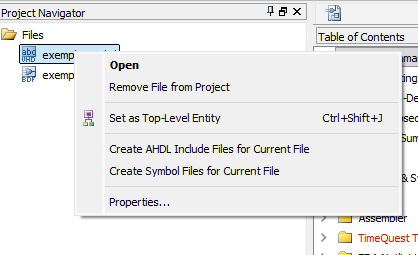
\includegraphics[width=0.4\textwidth]{Figs/tut_fig05.png}
	\end{figure}
\end{frame}



% --- SLIDE 3 ---
\begin{frame}{Passo 2: Atribuição de Pinos (Pinning)}
	Existem duas formas complementares de configurar os pinos da DE0-Nano:
	
	\begin{block}{Importação de Arquivo (.qsf)}
		\texttt{Assignments $\rightarrow$ Import Assignments...} \\
		Escolha o arquivo \textbf{DE0\_NANO.qsf} fornecido pela Terasic.
	\end{block}
	
	\begin{block}{Pin Planner (Ajuste Manual)}
		\texttt{Assignments $\rightarrow$ Pin Planner} \\
		Copie e cole os códigos (ex: PIN\_M1) para as portas correspondentes.
	\end{block}
	\begin{figure}
		%\includegraphics[width=0.6\textwidth]{pin_planner.png}
	\end{figure}
\end{frame}


\begin{frame}{Passo 2: Atribuição de Pinos (Pinning)}
	%  Existem duas formas complementares de configurar os pinos da DE0-Nano:
	%  
	%  \begin{block}{Importação de Arquivo (.qsf)}
		%    \texttt{Assignments $\rightarrow$ Import Assignments...} \\
		%    Escolha o arquivo \textbf{DE0\_NANO.qsf} fornecido pela Terasic.
		%  \end{block}
	%
	%  \begin{block}{Pin Planner (Ajuste Manual)}
		%    \texttt{Assignments $\rightarrow$ Pin Planner} \\
		%    Copie e cole os códigos (ex: PIN\_M1) para as portas correspondentes.
		%  \end{block}
	\begin{figure}
		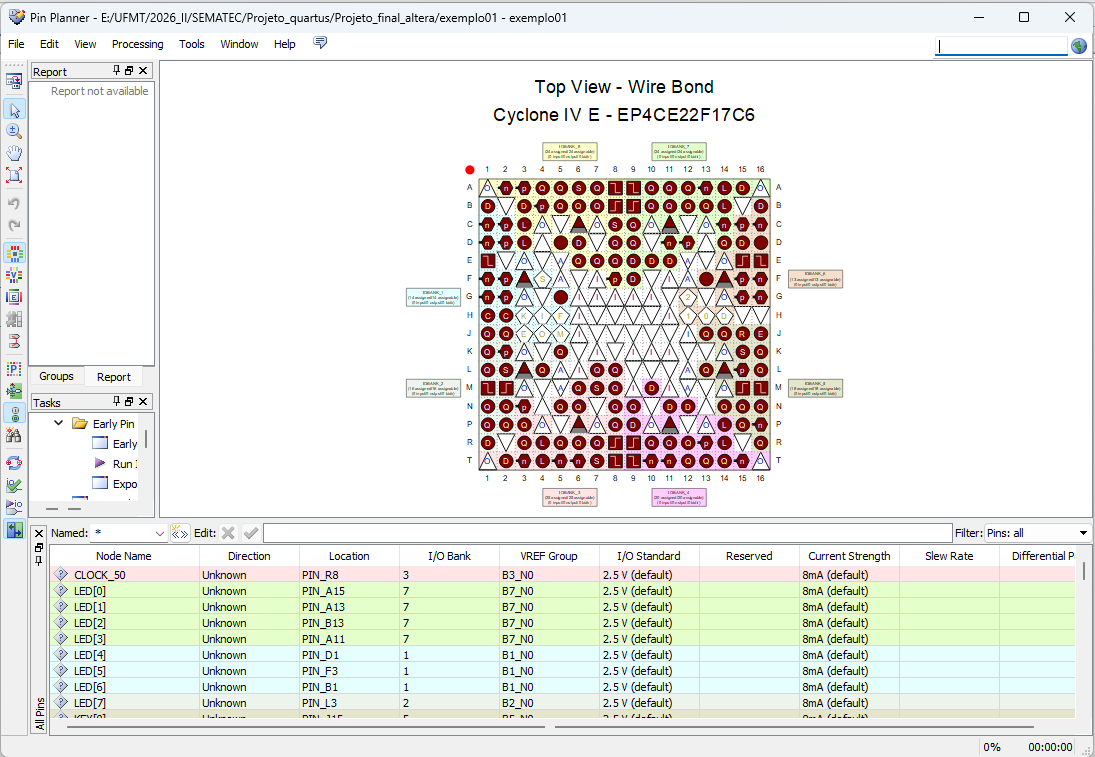
\includegraphics[width=0.6\textwidth]{Figs/tut_fig01.png}
	\end{figure}
\end{frame}




\begin{frame}{Passo 2: Atribuição de Pinos (Pinning)}
	%  Existem duas formas complementares de configurar os pinos da DE0-Nano:
	%  
	%  \begin{block}{Importação de Arquivo (.qsf)}
		%    \texttt{Assignments $\rightarrow$ Import Assignments...} \\
		%    Escolha o arquivo \textbf{DE0\_NANO.qsf} fornecido pela Terasic.
		%  \end{block}
	%
	%  \begin{block}{Pin Planner (Ajuste Manual)}
		%    \texttt{Assignments $\rightarrow$ Pin Planner} \\
		%    Copie e cole os códigos (ex: PIN\_M1) para as portas correspondentes.
		%  \end{block}
	\begin{figure}
		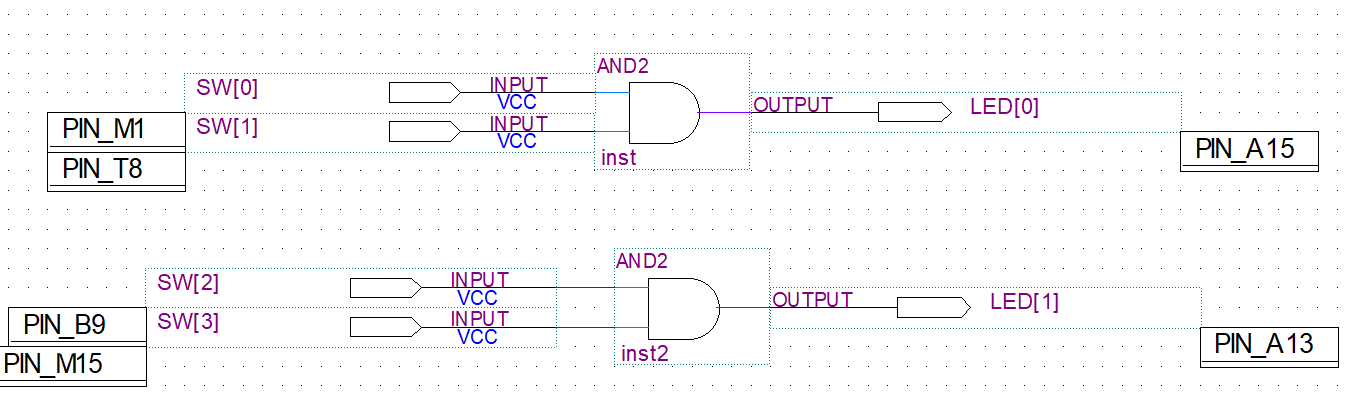
\includegraphics[width=0.6\textwidth]{Figs/tut_fig04.png}
	\end{figure}
\end{frame}








% --- SLIDE 4 ---
\begin{frame}{Passo 3: Convertendo para VHDL}
	Para fins de simulação e portabilidade, transformaremos o desenho em código:
	\begin{enumerate}
		\item Com o .bdf aberto: \texttt{File $\rightarrow$ Create/Update $\rightarrow$ Create HDL Design File...}
		\item Selecione \textbf{VHDL}.
		\item Adicione o arquivo .vhd gerado ao projeto (Botão direito em \textit{Files} $\rightarrow$ \textit{Add Files}).
		\item Remova o .bdf do projeto para evitar conflitos.
		\item Defina o novo .vhd como \textbf{Set as Top-Level Entity}.
		\item Clique em \textbf{Start Compilation}.
	\end{enumerate}
\end{frame}



\begin{frame}{Passo 3: Convertendo para VHDL}
	\begin{figure}
		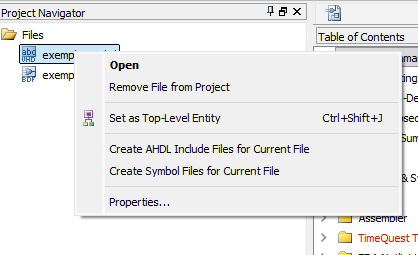
\includegraphics[width=0.6\textwidth]{Figs/tut_fig05.png}
	\end{figure}
\end{frame}







% --- SLIDE 5 ---
\begin{frame}{Passo 4: Gerando o Template de Testbench}
	O Quartus gera a wrapper do teste automaticamente:
	\begin{enumerate}
		\item \texttt{Processing $\rightarrow$ Start $\rightarrow$ Start Test Bench Template Writer}.
		\item O arquivo será criado em: \texttt{simulation/modelsim/nome\_projeto.vht}.
		\item Crie um novo arquivo VHDL no projeto e copie o conteúdo do .vht para ele.
		\item Renomeie a entidade de \texttt{exemplo\_vhd\_tst} para \texttt{exemplo\_tb}.
	\end{enumerate}
\end{frame}

















% --- SLIDE 6 ---
\begin{frame}[fragile]{Passo 5: Escrita dos Estímulos}
	No arquivo de testbench, identifique a seção de \textit{stimulus} e adicione o comportamento das chaves:
	
	\begin{lstlisting}[language=VHDL, basicstyle=\tiny]
		-- Exemplo de estimulos no Testbench
		SW <= "0000", 
		"0001" after 35 ns,
		"0010" after 55 ns,
		"0011" after 75 ns,
		"0101" after 105 ns,
		"1111" after 145 ns;
	\end{lstlisting}
	
	\begin{itemize}
		\item \textbf{DICA:} Mude o nome da instância (DUT) para facilitar a identificação.
	\end{itemize}
\end{frame}





% --- SLIDE 7 ---
\begin{frame}{Passo 6: Configurando o ModelSim}
	Ligar o Quartus ao simulador:
	\begin{enumerate}
		\item \texttt{Assignments $\rightarrow$ Settings $\rightarrow$ Simulation}.
		\item Em \textbf{Test Benches}, clique em \textbf{New}.
		\item \textbf{Test bench name:} exemplo\_tb.
		\item \textbf{Top level module:} exemplo\_tb.
		\item Adicione o arquivo .vhd do testbench e clique em OK.
	\end{enumerate}
	\begin{figure}
		%\includegraphics[width=0.6\textwidth]{settings_simulation.png}
	\end{figure}
\end{frame}




\begin{frame}{Passo 6: Configurando o ModelSim}
	%  Ligar o Quartus ao simulador:
	%  \begin{enumerate}
		%    \item \texttt{Assignments $\rightarrow$ Settings $\rightarrow$ Simulation}.
		%    \item Em \textbf{Test Benches}, clique em \textbf{New}.
		%    \item \textbf{Test bench name:} exemplo\_tb.
		%    \item \textbf{Top level module:} exemplo\_tb.
		%    \item Adicione o arquivo .vhd do testbench e clique em OK.
		%  \end{enumerate}
	\begin{figure}
		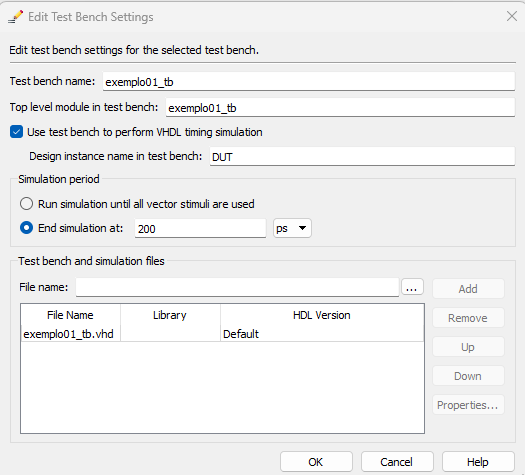
\includegraphics[width=0.5\textwidth]{Figs/tut_fig17.png}
	\end{figure}
\end{frame}












% --- SLIDE 8 ---
\begin{frame}{Passo 7: Executando a Simulação}
	\begin{itemize}
		\item Vá em \texttt{Tools $\rightarrow$ Run Simulation Tool $\rightarrow$ RTL Simulation}.
		\item O ModelSim abrirá automaticamente.
	\end{itemize}
	
	\begin{block}{Dica de Produtividade (Console ModelSim)}
		Para rodar novamente após mudar o código:
		\begin{enumerate}
			\item Use a seta para cima no console do ModelSim.
			\item Procure o comando: \texttt{do exemplo\_run\_msim\_rtl\_vhdl.do}.
		\end{enumerate}
	\end{block}
\end{frame}




\begin{frame}{Passo 7: Executando a Simulação}
	\begin{figure}
		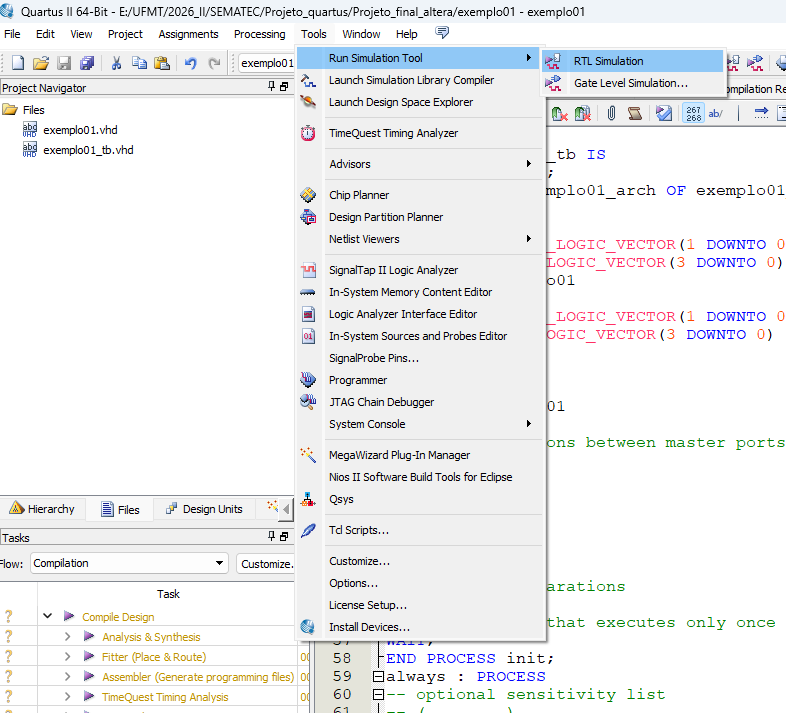
\includegraphics[width=0.5\textwidth]{Figs/tut_fig06.png}
	\end{figure}
\end{frame}















% --- SLIDE 9 ---
\begin{frame}{Passo 8: Ajustes Finos (Ondas e Tempo)}
	\begin{enumerate}
		\item No ModelSim, organize as ondas e salve como \textbf{wave.do}.
		%    \item Edite o arquivo \texttt{.do} principal na pasta \textit{simulation/modelsim}:
		%    \item Adicione o comando \texttt{do wave.do}.
		%    \item Aumente o tempo de simulação (ex: \texttt{run 500 ns}).
		%    \item Altere a representação (Radix) para Decimal ou Hexadecimal clicando com o botão direito no sinal.
	\end{enumerate}
	
	\begin{figure}
		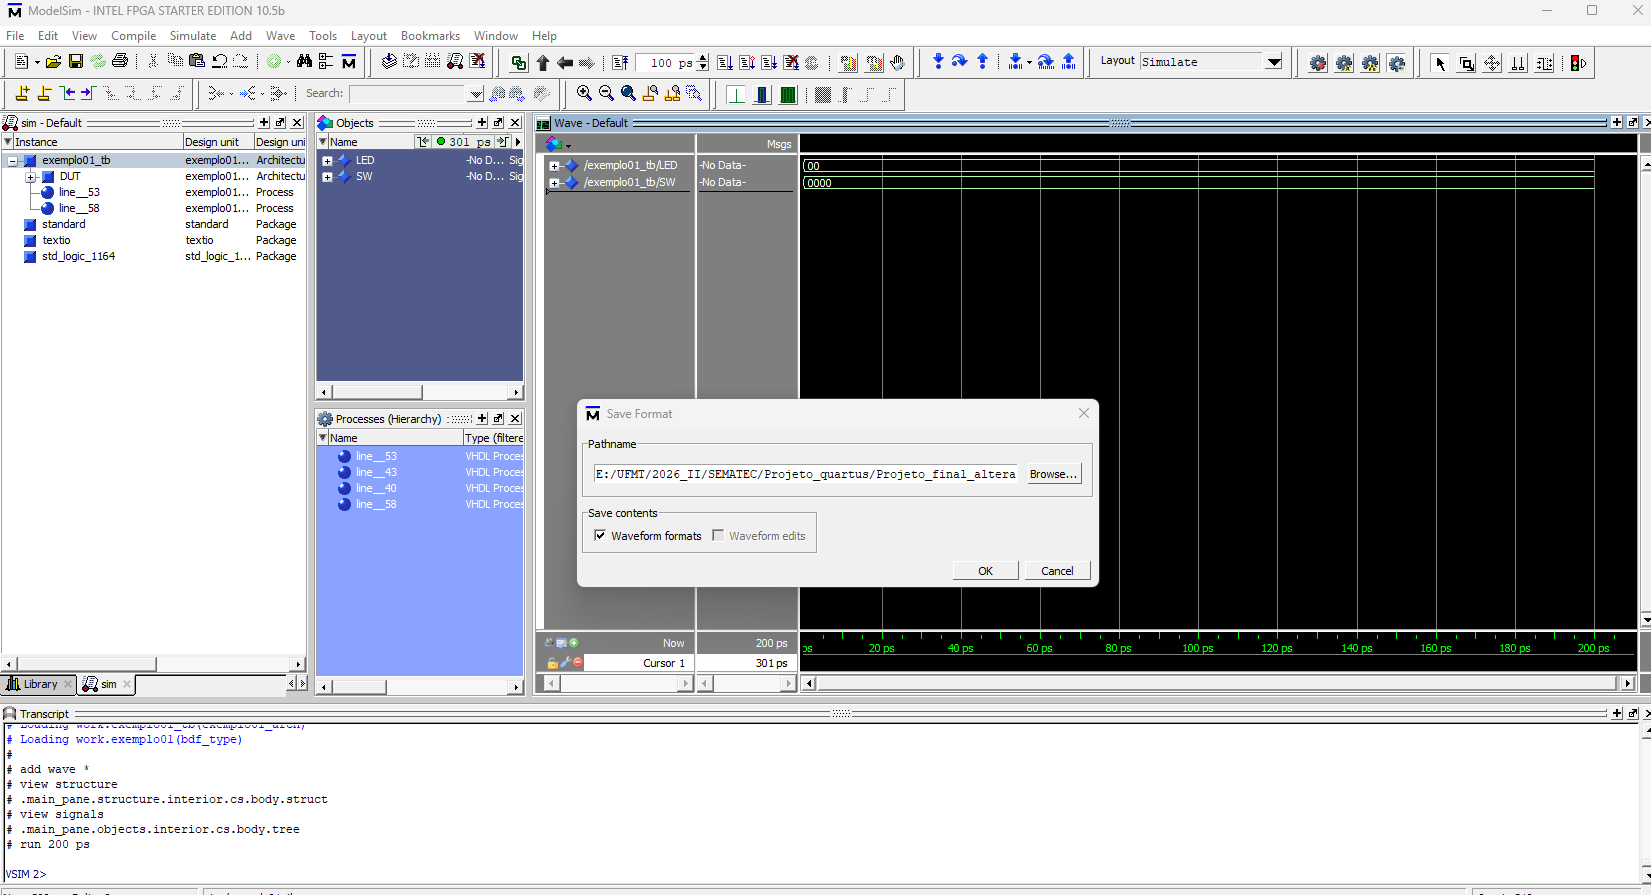
\includegraphics[width=0.8\textwidth]{Figs/tut_fig11.png}
	\end{figure}
	
	
\end{frame}





\begin{frame}{Passo 8: Ajustes Finos (Ondas e Tempo)}
	
	\begin{enumerate}
		% \item No ModelSim, organize as ondas e salve como \textbf{wave.do}.
		\item Edite o arquivo \texttt{.do} principal na pasta \textit{simulation/modelsim}:
		%    \item Adicione o comando \texttt{do wave.do}.
		%    \item Aumente o tempo de simulação (ex: \texttt{run 500 ns}).
		%    \item Altere a representação (Radix) para Decimal ou Hexadecimal clicando com o botão direito no sinal.
	\end{enumerate}
	
	
	\begin{figure}
		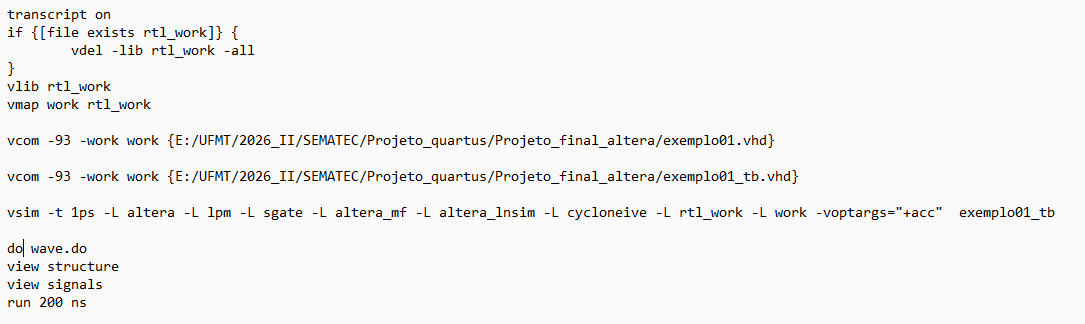
\includegraphics[width=0.9\textwidth]{Figs/tut_fig10.png}
	\end{figure}
\end{frame}


\begin{frame}{Passo 8: Ajustes Finos (Ondas e Tempo)}
	
	\begin{enumerate}
		% \item No ModelSim, organize as ondas e salve como \textbf{wave.do}.
		%\item Edite o arquivo \texttt{.do} principal na pasta \textit{simulation/modelsim}:
		% \item Adicione o comando \texttt{do wave.do}.
		% \item Aumente o tempo de simulação (ex: \texttt{run 500 ns}).
		\item Altere a representação (Radix) para Decimal ou Hexadecimal clicando com o botão direito no sinal.
	\end{enumerate}
	
	
	\begin{figure}
		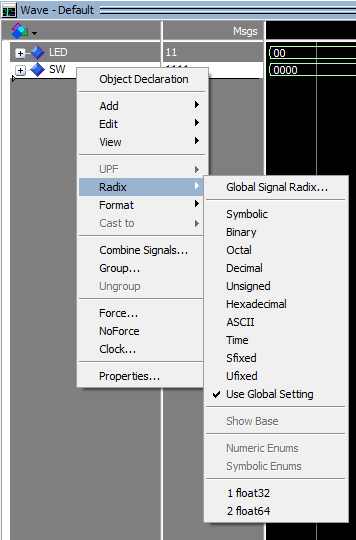
\includegraphics[width=0.3\textwidth]{Figs/tut_fig16.png}
	\end{figure}
\end{frame}










%\begin{frame}{Passo 8: Ajustes Finos (Ondas e Tempo)}
%
%  \begin{enumerate}
	%   % \item No ModelSim, organize as ondas e salve como \textbf{wave.do}.
	%    %\item Edite o arquivo \texttt{.do} principal na pasta \textit{simulation/modelsim}:
	%    \item Adicione o comando \texttt{do wave.do}.
	%    \item Aumente o tempo de simulação (ex: \texttt{run 500 ns}).
	%    \item Altere a representação (Radix) para Decimal ou Hexadecimal clicando com o botão direito no sinal.
	%  \end{enumerate}
%  
%  
%     \begin{figure}
	%    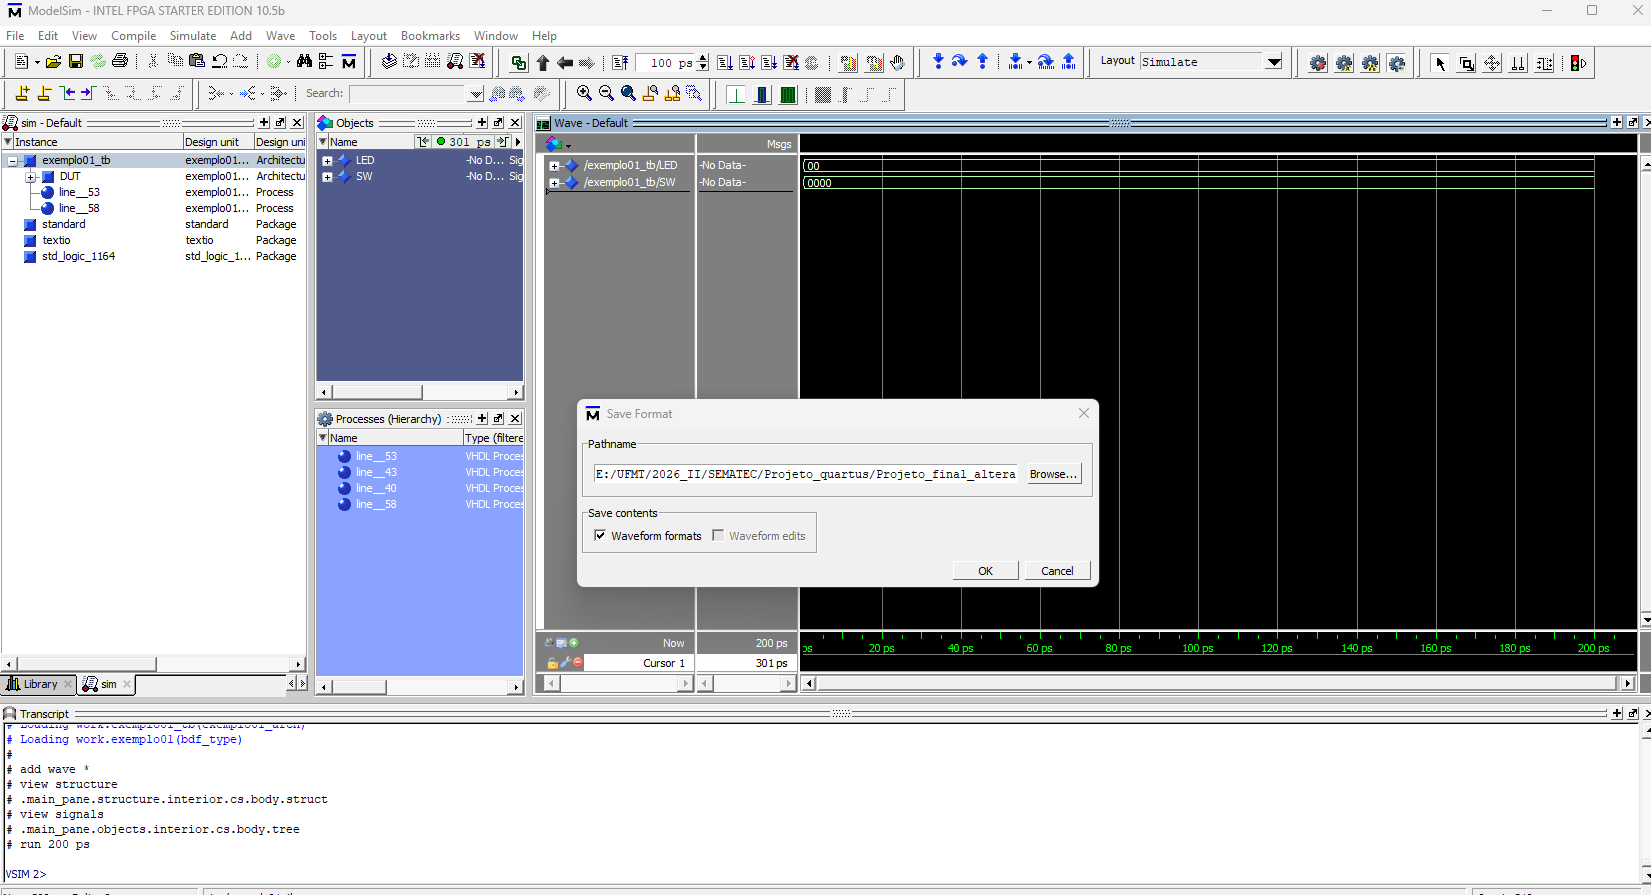
\includegraphics[width=0.5\textwidth]{Figs/tut_fig11.png}
	%  \end{figure}
%\end{frame}














% --- SLIDE 10 ---
\begin{frame}{Finalização}
	\begin{enumerate}
		\item Verifique se as saídas LED[0] e LED[1] obedecem à lógica AND das chaves.
		\item Após validar no simulador, volte ao Quartus.
		\item Conecte a placa DE0-Nano via USB.
		\item \texttt{Tools $\rightarrow$ Programmer} e clique em \textbf{Start}.
	\end{enumerate}
	
	\begin{figure}
		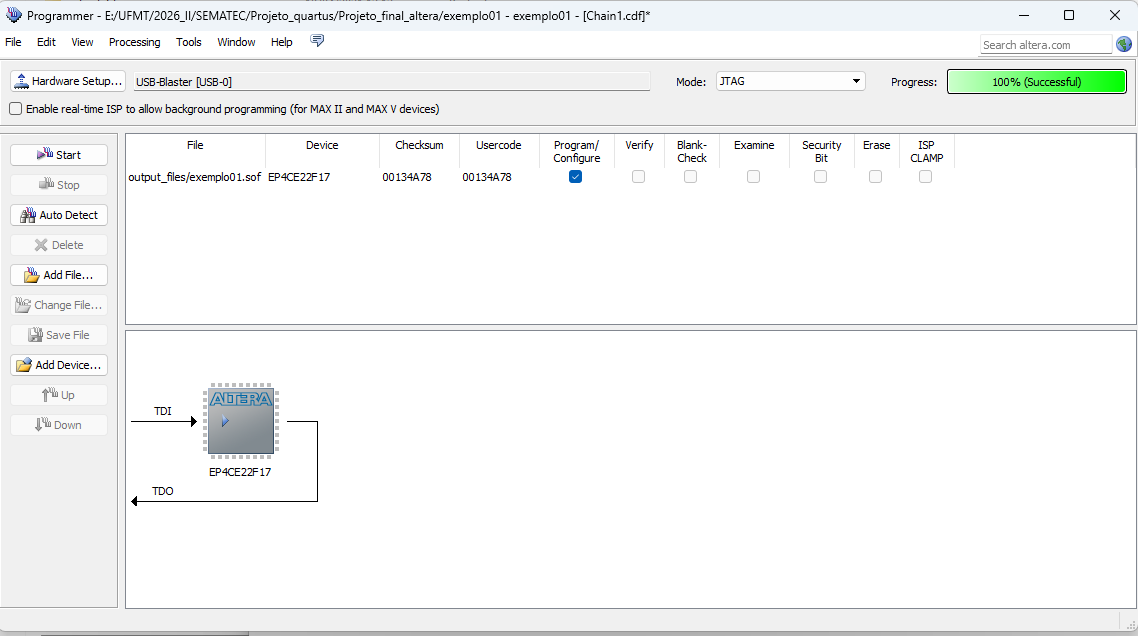
\includegraphics[width=0.5\textwidth]{Figs/tut_fig03.png}
	\end{figure}
	
	
	\begin{center}
		\textbf{Parabéns! Seu hardware está rodando.}
	\end{center}
\end{frame}



\end{document}
